%%%%%%%%%%%%%%%%%%%
%  placeholders
%%%%%%%%%%%%%%%%%%%

% chair name not allowed at Department of Informatics
% remove \phantom{} if you want the chair name on the cover
\newcommand{\chair}{{Lehrstuhl f\"ur Integrierte Systeme}}
\newcommand{\faculty}{Fakult\"at f\"ur Elektrotechnik und Informationstechnik}
\newcommand{\uni}{Technische Universit\"at M\"unchen}
\newcommand{\studycourse}{Digital systems and FPGA engineering}

\newcommand{\authorname}{Mohammed Adib Obaid}
\newcommand{\city}{Munich}

\newcommand{\worktype}{Internship in \studycourse}
\newcommand{\titleFirstLanguage}{Implementation of an FIR Filter on FPGA for Laser Line Extraction from Pixel Data}
% German & English needed at Department of Informatics
\newcommand{\titleForeignLanguage}{}

\newcommand{\supervisor}{Arne Kreddig}
\newcommand{\advisor}{Arne Kreddig}

% set date manually or use \today
\newcommand{\submissionDate}{\today}



%%%%%%%%%%%%%%%%%%%
%    settings
%%%%%%%%%%%%%%%%%%%

% quick settings
\def\printstyle{twoside} % set to {twoside} for printing, else {oneside}
%\def\monochromeCover{} % uncomment if you prefer a black TUM logo on the cover
% \def\monochromeCoverInside{} % uncomment if you prefer a black TUM logo on the inside cover page

% complete settings & packages: see settings.text
%%%%%%%%%%%%%%%%%%%
% essentials
%%%%%%%%%%%%%%%%%%%

% use the scrbook KOMA document class
\documentclass[	pdftex, 		%
	a4paper, 		% DIN A4 format
	titlepage,		% separate title page
	%draft,			% draft version, no figures in PDF!
	final,			% final version
	\printstyle ,		% see \def in main document (oneside or twoside)
	11pt,			% font size
	DIV=calc,
]{scrbook}

\setkomafont{disposition}{\normalfont\bfseries}
\usepackage{scrhack}

% page geometry - define custom if needed...
\def\coverborderleft{20mm} % needed for title page - update: Druck mit Pappumschlag braucht's eher nicht
\usepackage[left=30mm , right=30mm, top=30mm, bottom=30mm]{geometry}

% typesetting
\usepackage{palatino} 				% Palatino font with sans-serif \sffamily Helvetica
\usepackage[utf8]{inputenc} 			% Umlaute
\usepackage[T1]{fontenc}			% extended character set
\parindent0pt           			% no indentation of the first line
\parskip1ex             			% gap between paragraphs
\usepackage{setspace}				% package for line spacing settings
\singlespacing					% 1,0
%\onehalfspacing				% 1,5
%\doublespacing					% 2,0

% language for automated stuff, like "List of Figures" or "Abbildungsverzeichnis"
\usepackage[english]{babel}
%\usepackage[german=quotes]{csquotes} % Deutsche Anführungszeichen

% BibTex
% \usepackage{natbib}
\bibliographystyle{IEEEtran}



%%%%%%%%%%%%%%%%%%%
% figures & co
%%%%%%%%%%%%%%%%%%%

% graphics and figures
\usepackage{graphicx, tikz, pgfplots}
\graphicspath{{images/}} % additional path(s) for loading images
\usepackage{rotating} % needed for \begin{sidewaysfigure} ... 

% insert PDF files
\usepackage{pdfpages}
% settings for PDF Pages to accept additonal versioned PDF files
\pdfminorversion=6
\pdfcompresslevel=9
\pdfobjcompresslevel=9

% define custom colors
\usepackage{xcolor}
\definecolor{gray1}{gray}{0.92}
\definecolor{darkgreen}{rgb}{0,0.5,0}
\definecolor{urlLinkColor}{rgb}{0,0,0.5}
\definecolor{LinkColor}{rgb}{0,0,0}
\definecolor{ListingBackground}{rgb}{0.85,0.85,0.85}

\usepackage{color}
\definecolor{LinkColor}{rgb}{0.1,0.1,0.1}
\definecolor{ListingBackground}{rgb}{0.98,0.98,0.98}
\definecolor{gray}{rgb}{0.4,0.4,0.4}
\definecolor{darkblue}{rgb}{0.0,0.0,0.6}
\definecolor{cyan}{rgb}{0.0,0.6,0.6}



%%%%%%%%%%%%%%%%%%%
% layout tools
%%%%%%%%%%%%%%%%%%%

% for \textblock on title page
\usepackage[absolute]{textpos}
%\setlength{\TPHorizModule}{1mm}
%\setlength{\TPVertModule}{\TPHorizModule}

% TUM Corporate Design definitions taken from official templates (tum.de/cd)
\newcommand{\UniversitaetLogoBreite}{19mm}
\newcommand{\UniversitaetLogoHoehe}{1cm}
\definecolor{UniversitaetFarbe}{RGB}{0,101,189}

% blindtext generator
\usepackage{lipsum}

% advanced conditionals
\usepackage{pdftexcmds}


%%%%%%%%%%%%%%%%%%%
% math
%%%%%%%%%%%%%%%%%%%

\usepackage{amssymb}
\usepackage{amsmath}
% custom argmin, argmax
\newcommand{\argmax}[1]{\underset{#1}{\operatorname{arg}\,\operatorname{max}}\;}
\newcommand{\argmin}[1]{\underset{#1}{\operatorname{arg}\,\operatorname{min}}\;}



%%%%%%%%%%%%%%%%%%%
% code listings
%%%%%%%%%%%%%%%%%%%

\usepackage{listings}
\lstloadlanguages{TeX, C++, XML, Matlab, Java, Python, C} % add languages if needed 
\lstset{%
	language=[LaTeX]TeX,     %
	numbers=left,            % line numbers left
	stepnumber=1,            % number every line
	numbersep=5pt,           % distance of line numbers to the code
	numberstyle=\tiny,       % size of the line numbers
	breaklines=true,         % break lines if necessary
	breakautoindent=true,    % indent lines after line breaks
	postbreak=\space,        % line break at spaces
	tabsize=2,               % size of tab indentation
	basicstyle=\small\ttfamily,
	showspaces=false,        % don't show spaces
	columns=fullflexible,
	showstringspaces=false,  % ...also not in 'strings' / "strings"
	extendedchars=true,      % show all Latin1 chars
	backgroundcolor=\color{ListingBackground} % background color of the listing
}

% captions for listings
\usepackage{caption}
\DeclareCaptionFont{white}{\color{white}}
\DeclareCaptionFormat{listing}{\colorbox[cmyk]{0.43, 0.35, 0.35,0.01}{\parbox{\textwidth}{\hspace{15pt}#1#2#3}}}
\captionsetup[lstlisting]{format=listing,labelfont=white,textfont=white, singlelinecheck=false, margin=0pt, font={footnotesize}}



%%%%%%%%%%%%%%%%%%%
% header & footer
%%%%%%%%%%%%%%%%%%%

\usepackage{fancyhdr}
\pagestyle{fancy}
\fancyhead{}
\fancyfoot{}
\renewcommand{\headrulewidth}{0.4pt} % line for header - 0.0pt = no line
\renewcommand{\footrulewidth}{0.0pt} % line for footer - 0.0pt = no line

\renewcommand{\chaptermark}[1]{\markboth{\thechapter\quad#1}{}}
\renewcommand{\sectionmark}[1]{\markright{\thesection\quad#1}}

\fancyhead[LO]{\textit{\rightmark}}
\fancyhead[RO]{\textit{\thepage}}

\def\twoside{twoside} % macro needed
\ifx \printstyle \twoside
	% adapt footers and headers if two-sided
	\fancyhead[LE]{\textit{\thepage}}
	\fancyhead[RE]{\textit{\rightmark}}
\fi



%%%%%%%%%%%%%%%%%%%
% hyperref
%%%%%%%%%%%%%%%%%%%

\usepackage[
	pdftitle={\titleFirstLanguage},
	pdfauthor={\authorname},
	pdfsubject={\titleFirstLanguage},
	pdfcreator={Adib},
	pdfkeywords={Abschlussarbeit, Thesis, TUM},
	pdfpagemode=UseOutlines,%                                  
	pdfdisplaydoctitle=true,%                                  
	pdflang=de%                                              
]{hyperref}

\hypersetup{%
	colorlinks=true,%        colored links without border
	linkcolor=LinkColor,%    
	citecolor=LinkColor,%    
	filecolor=LinkColor,%    
	menucolor=LinkColor,%    
	urlcolor=LinkColor,%     
	bookmarksnumbered=true%  
}

\usepackage{dirtree}
\usepackage{forest}
\usepackage{svg}
\usepackage{url}
 


%%%%%%%%%%%%%%%%%%%
%  main document
%%%%%%%%%%%%%%%%%%%


\pgfplotsset{compat=1.15}
\begin{document}

\frontmatter
% first part of document before actual content

\begin{titlepage}

% Dreizeiler:
\begin{textblock*}{\textwidth}(\coverborderleft, 2cm)%        	
    	\setlength{\baselineskip}{11pt}%
    	\ifx \monochromeCover \undefined
        	\textcolor{UniversitaetFarbe} { %
        	\fontsize{9}{11}\selectfont%
        	\sffamily \chair\\%
        	\sffamily \faculty\\%
        	\sffamily \uni }
    \else
        	\textcolor{black} { %
        	\fontsize{9}{11}\selectfont%
        	\sffamily \chair\\%
        	\sffamily \faculty\\%
        	\sffamily \uni }
    \fi
\end{textblock*}%

% TUM logo
\begin{textblock*}{\UniversitaetLogoBreite}[1,0](\paperwidth - 2cm, 2cm)%
		\ifx \monochromeCover \undefined
        	
\includegraphics{images/TUM_Logos/TUM_blau.pdf}%
        \else
        	
\includegraphics{images/TUM_Logos/TUM_schwarz.pdf}%
        \fi
\end{textblock*}%

% title text
\begin{textblock*}{\paperwidth - \coverborderleft - 2cm}(\coverborderleft , 8cm)% 
\raggedright %no hyphenation here
{\sffamily \Large \worktype}\\
{\sffamily \huge \titleFirstLanguage \par} %~\\[2mm]
\vspace{1cm}
\sffamily \Large \textbf{\authorname}\\
\end{textblock*}

~\\ % do not remove
\end{titlepage}
% \begin{titlepage}

% Dreizeiler:
\begin{textblock*}{\textwidth}(\coverborderleft, 2cm)%        	
    	\setlength{\baselineskip}{11pt}%
    	\ifx \monochromeCoverInside \undefined
        	\textcolor{UniversitaetFarbe} { %
        	\fontsize{9}{11}\selectfont%
        	\sffamily \chair\\%
        	\sffamily \faculty\\%
        	\sffamily \uni }
    \else
        	\textcolor{black} { %
        	\fontsize{9}{11}\selectfont%
        	\sffamily \chair\\%
        	\sffamily \faculty\\%
        	\sffamily \uni }
    \fi
\end{textblock*}%

% TUM logo
\begin{textblock*}{\UniversitaetLogoBreite}[1,0](\paperwidth - 2cm, 2cm)%
		\ifx \monochromeCoverInside \undefined
        	
\includegraphics{images/TUM_Logos/TUM_blau.pdf}%
        \else
        	
\includegraphics{images/TUM_Logos/TUM_schwarz.pdf}%
        \fi
\end{textblock*}%

% title in German and English with additional infos
\begin{textblock*}{\paperwidth - \coverborderleft -2cm}(\coverborderleft, 8cm)% 
\raggedright %no hyphenation here
{\sffamily \Large \worktype}\\
{\sffamily \huge \titleFirstLanguage \par}
\vspace{1cm}
{\sffamily \huge \titleForeignLanguage \par}
\end{textblock*}
\begin{textblock*}{\paperwidth - \coverborderleft - 2cm}(\coverborderleft, \paperheight - 5cm)% 
\begin{tabular}{l l}
\sffamily Author: & \sffamily \authorname \\
\sffamily Supervisor: & \sffamily \supervisor \\
\sffamily Advisors: & \sffamily \advisor \\
\sffamily Submission Date: & \sffamily \submissionDate
\end{tabular}
\end{textblock*}

~\\ % do not remove
\end{titlepage} % needed at Department of Informatics

% \chapter{Eidesstattliche Erkl\"arung}
Ich versichere hiermit, dass ich diese Master's Thesis selbständig verfasst und nur die angegebenen Quellen und Hilfsmittel verwendet habe.
\\[1cm]
I confirm that this master's thesis is my own work and I have documented all sources and material used.
\\[6ex]

\city, \submissionDate

\vspace{1.5cm}
\rule[-0.2cm]{5cm}{0.5pt}

\textsc{\authorname} 

\chapter{Abstract}\label{Abstract}

Current 3D laser line scanners have precision in the range of a micrometer. These scanners work on the principle of laser triangulation and use a camera chip in the receive path. The captured pixel data is then processed on an FPGA to generate 3D profile data. In order to do this, the laser line, as seen by the camera, must be extracted from the pixel data. For this purpose, several methods have been proposed. One of these methods employs an FIR filter to calculate the derivative of the incoming pixel stream orthogonally to the laser line direction. Afterwards, the zero crossing of this derivative is detected. The position of the zero crossing marks the position of the laser line in the camera image. From this position, the distance of the laser scanner to the scanned object can be derived.

This project was implemented using VHDL for the digital modules. In addition to that, Python tools were developed to assist in system modeling, simulation and test vector generation. The report highlights the proposed solution, an overview of the scripts and tools developed to assist in the system architecture design, a comprehensive look at each module, and finally a look at how the system can be improved.

% \chapter{Acknowledgements}

I would like to thank Michael Grupp for this \LaTeX\ template.

\lipsum[1-2]


\tableofcontents


\mainmatter
% include chapter files here or write your text directly here

\chapter{Problem definition and the Proposed solution}

\section{3D Laser Line Scanners}


3D laser line scanners work on the principle of laser triangulation and use a camera chip in the receive path. The setup shown in Figure \ref{fig:laser_line_setup} consists of a camera sensor with an angle $\alpha$ from the vertical line, and a laser line source directed on top of the object. When the laser is cast onto the object, the laser line is captured by the camera sensor.


\begin{figure}[h]
    \centering
    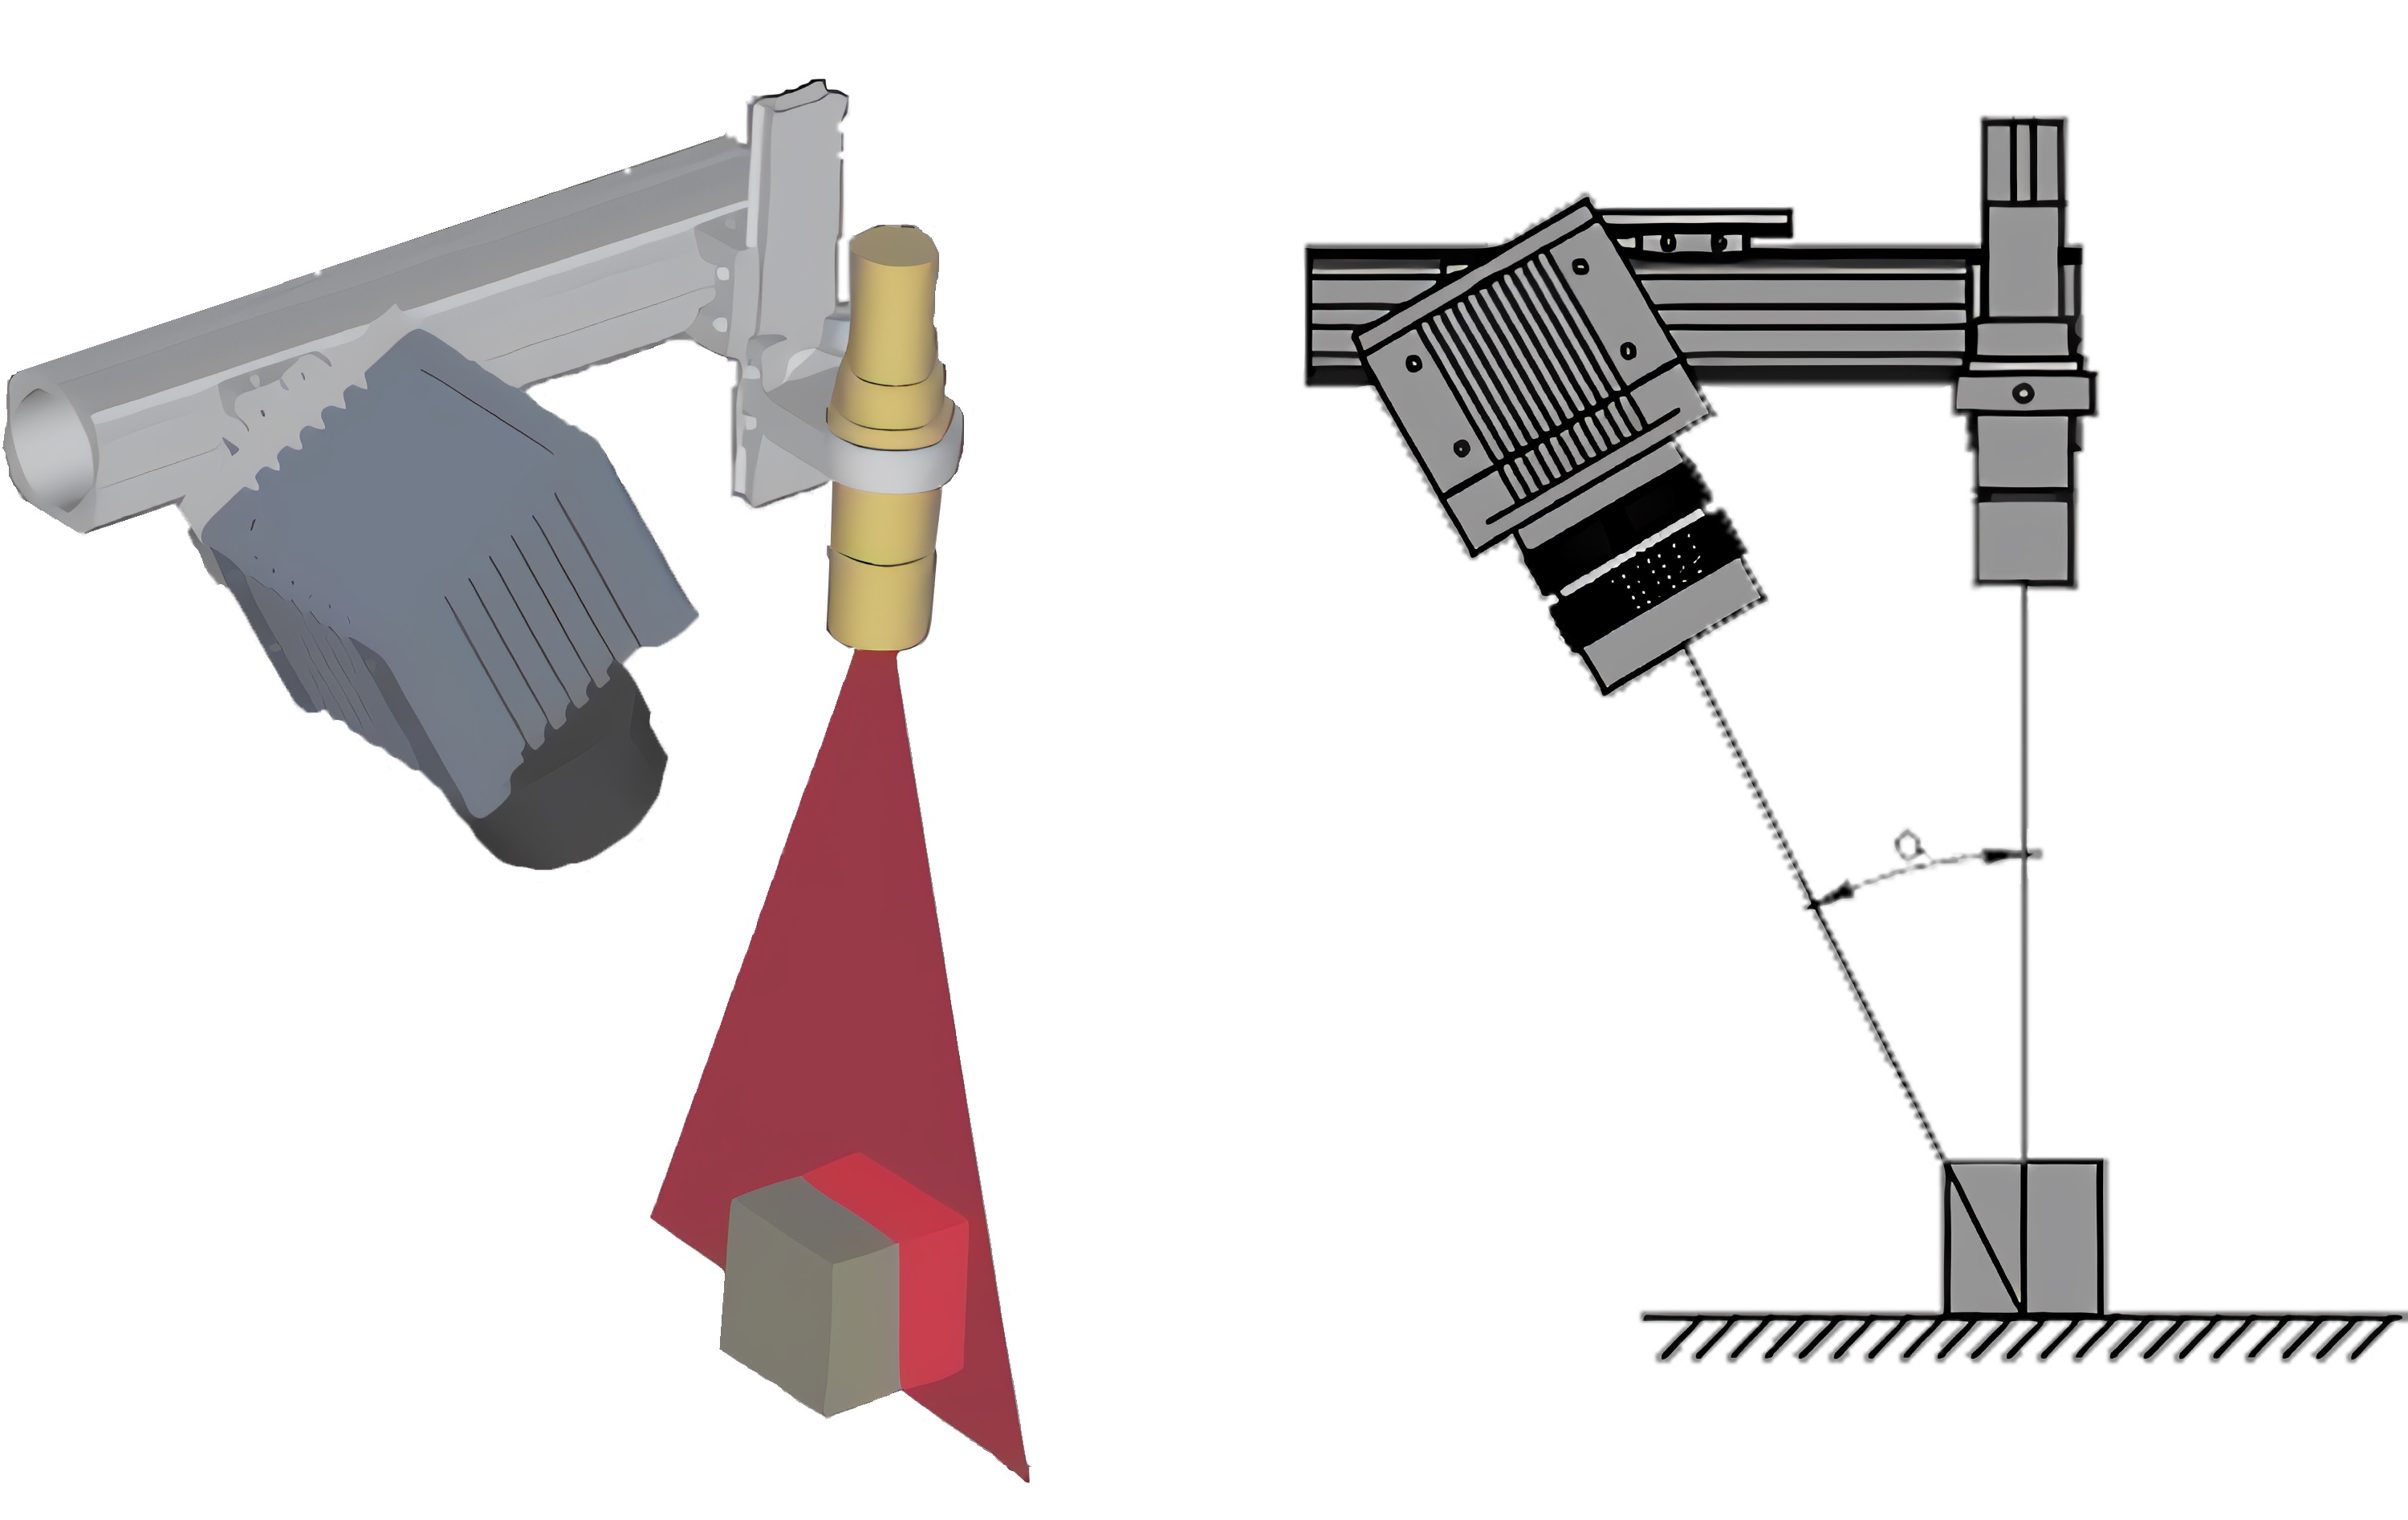
\includegraphics[width=0.8\textwidth]{laser_line_setup_upscaled_nn.jpg}
    \caption{3D laser line scanning setup \cite{method_presentation}}
    \label{fig:laser_line_setup}
\end{figure}


The captured pixel data is then processed on an FPGA to generate 3D profile data. In order to do this, the laser line, as seen by the camera, must be extracted from the pixel data. For this purpose, several methods have been proposed to extract the line data from the captured image. One of these methods employs an FIR filter to calculate the derivative of the incoming pixel stream orthogonally to the laser line direction. Afterwards, the zero crossing of this derivative is detected. The position of the zero crossing marks the position of the laser line in the camera image. From this position, the distance of the laser scanner to the scanned object can be derived.


\section{The proposed solution}


\begin{figure}[h]
    \centering
    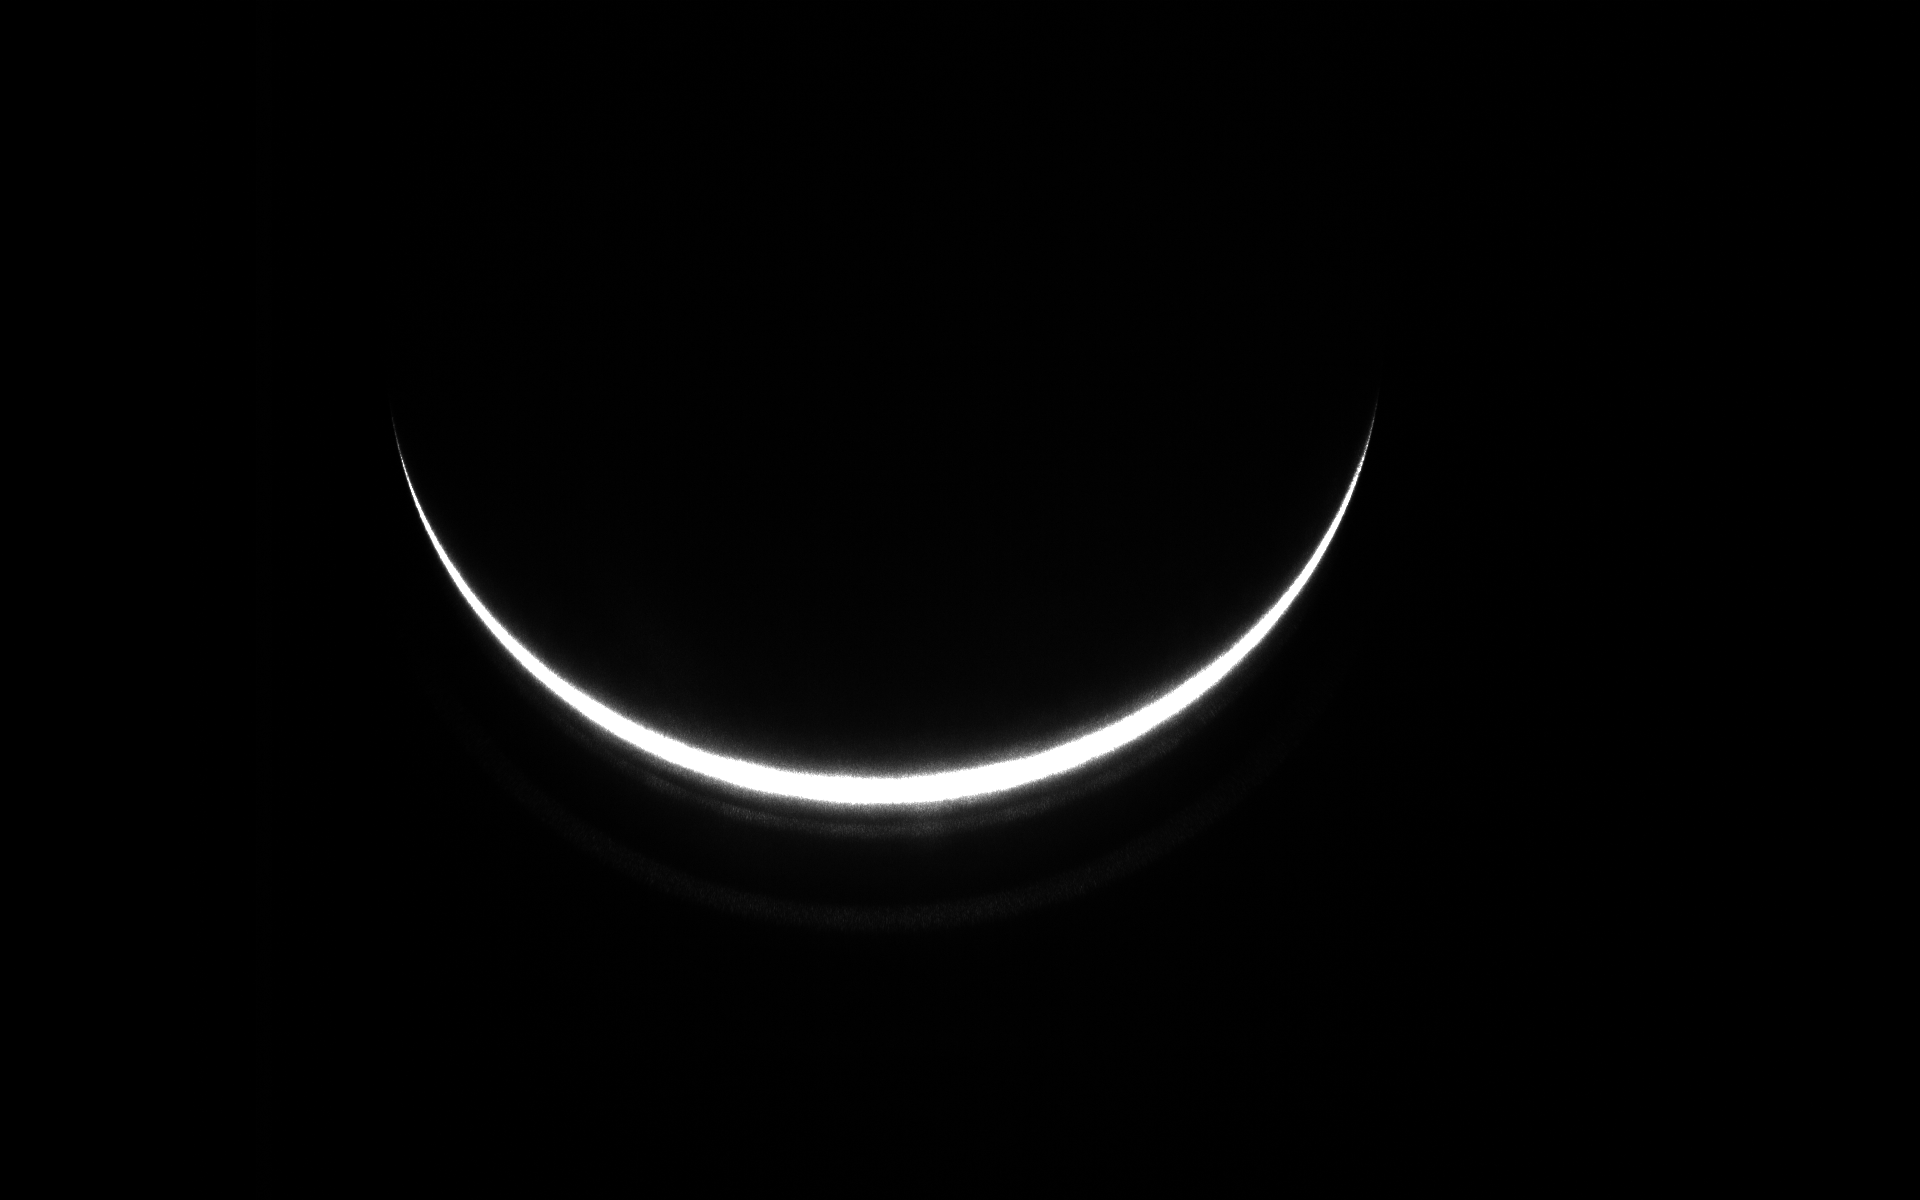
\includegraphics[width=0.8\textwidth]{sphere_laser_line.png}
    \caption{Pixel data of a laser line projected onto a spherical object}
    \label{fig:sphere_laser_line}
\end{figure}


Figure \ref{fig:sphere_laser_line} shows pixel data of a laser line cast onto a spherical shaped object. As shown in the image, the reflected laser line from the scanned object is shown as a white line in the pixel data.

The goal in this project is to extract the white line from the pixel data, and the proposed method is to process each vertical pixel line individually as shown in Figure \ref{fig:sphere_laser_line_pixel_column}. The extracted data is orthogonal to the laser line. The column data forms a gaussian distribution curve where the point of maximum intensity should point to the middle of the white laser line.


\begin{figure}[h]
    \centering
    \includesvg[width=1\textwidth]{sphere_laser_line_column.svg}
    \caption{Pixel column distribution}
    \label{fig:sphere_laser_line_pixel_column}
\end{figure}

There are several methods of exctracting the point of maximum intensity from a gaussian distribution curve. Figure \ref{fig:extraction_methods}  shows an overview of three maximum point finding methods \cite{method_presentation}. The first method is looking for the point of maximum intensity of the incoming data. Second method is to accept any point with an intensity higher than a preset threshold. Afterwars, the center position between these points is selected \cite{7794138}. Third method is to find the center of gravity of the area under the Gaussian curve \cite{7794138}. In this project, a fourth method is explored, where the derivative of the gaussian curve formed by the pixel intensity is taken. A zero-crossing in the first derivative occurs at the same position of the extremum of the incoming pixel data.


\begin{figure}[h]
    \centering
    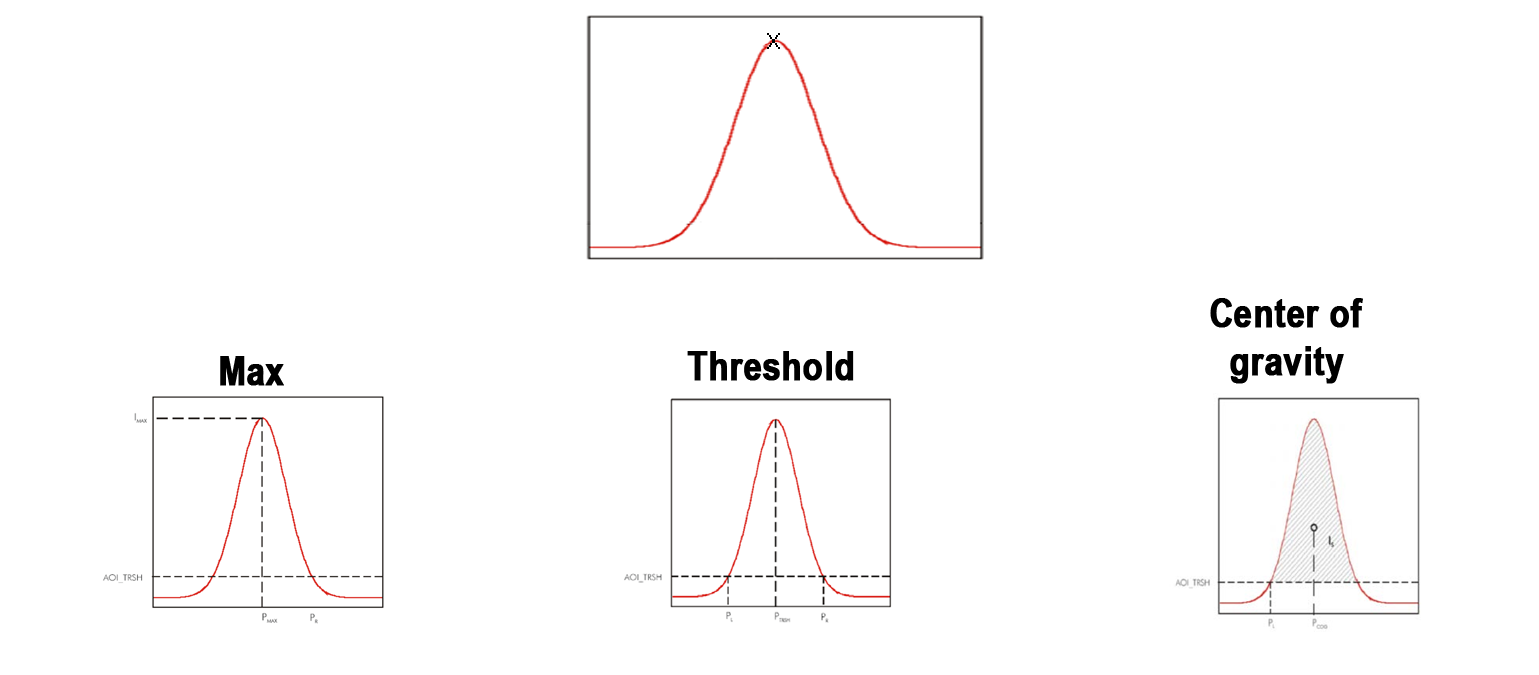
\includegraphics[width=1\textwidth]{extraction_methods.png}
    \caption{Extraction methods \cite{method_presentation}}
    \label{fig:extraction_methods}
\end{figure}

Figure \ref{fig:diff_flow} shows how the gaussian distribution curve would look like after taking its first derivative. The resulting differentiated dataset crosses from a positive value to a negative value at the point of maximum intensity. %In the example shown in \ref{fig:diff_flow} the differentiated data stagnates around zero for a bit then becomes negative because the image had a high exposure time which made the laser line over saturated.


\begin{figure}[h]
    \centering
    \includesvg[width=1\textwidth]{data_to_diff_flow.svg}
    \caption{Image data to differentiated data}
    \label{fig:diff_flow}
\end{figure}


The processing system is composed of two main parts: The filters and the zero-crossing detector. The filtering part of the system has two jobs: it needs to smooth out the data and to differentiate the gaussian curve. While the zero-crossing part of the system will detect a positive to negative going zero-crossing position, this would mark the position of the laser line in the received pixel column.




\subsection{FIR filters}

Several filter setups has been experimented with during the initial system development phase. The FIR filter setup that was implemented in VHDL in this project consists of two FIR filters, a smoothing filter and a differentiation filter. Both filters are 5 taps Savitzky–Golay filters.

The filter sizes were chosen to limit the resource usage in the final design, as increasing the number of taps didn't provide enough extra smoothing to justify the extra FPGA area needed to implement it as shown in Figure \ref{fig:smoothing_filter_tap_cmp}


\begin{figure}[h]
    \centering
    \includesvg[width=1\textwidth]{smoothing_ex_1.svg}
    \caption{Smoothing filter tap comparison}
    \label{fig:smoothing_filter_tap_cmp}
\end{figure}


The differentiation filter is a 5-tap first order Savitzky–Golay filter. Figure \ref{fig:data_through_filters} shows how the data looks like after passing both filters, as shown in the third sub-plot there is a zero-crossing at the point of maximum intensity shown in the first and second subplots.

\begin{figure}[h]
    \centering
    \includesvg[width=0.8\textwidth]{data_through_filters.svg}
    \caption{(a) Raw pixel data, (b) Smoothing filter output, (c) Differentiation filter output}
    \label{fig:data_through_filters}
\end{figure}

Since pixel data is 8-bits wide and the current system does operations on signed 16-bit integers then there was no need for normalization for filter results. The filter coefficients are as shown in \eqref{fil_coeff}:

\begin{equation}\label{fil_coeff}
    \begin{aligned}
        smoothing filter \Leftarrow \{ -3, 12, 17, 12, -3 \} \\
        differentiation filter \Leftarrow \{ 2, 1, 0, -1, -2 \}
    \end{aligned}
\end{equation}



\subsection{Zero crossing}

There are several methods to find the position at which a positive-to-negative going zero-crossing has happened. One method is to search for the pattern $\{ positive, 0, negative\} $, but the issue with this approach is that oftentimes the pixel data platues at the max value for several pixels before going down again which results in an extended amount of zeros at the zero-crossing as shown in Figure \ref{fig:zero_crossing_extended_zeros}

\begin{figure}[h]
    \centering
    \includesvg[width=0.7\textwidth]{zero_crossing_extended_zeros.svg}
    \caption{Several zero values at the zero-crossing position}
    \label{fig:zero_crossing_extended_zeros}
\end{figure}

A solution to this problem would be supporting varrying numbers of zeros in the middle of the matching pattern. This solution is not robust for an FPGA application as it requires going through the same set of data multiple times.

Another method to detect zero-crossings is to find the maximum value and the minimum value, ensure that the max value's index is less than the min value's index, then find the index in the middle. Generally this method provides accurate results for images that aren't very noisy.


\begin{figure}[h]
    \centering
    \includesvg[width=0.9\textwidth]{zero_crossing_midpoint.svg}
    \caption{Zero-crossing at midpoint of two peaks}
    \label{fig:zero_crossing_midpoint}
\end{figure}

Figure \ref{fig:zero_crossing_midpoint} shows how the zero-crossing can be located using the midpoint between the two peaks. Eq.\eqref{zero_index_eq} shows the equation used to find the zero-crossing index. $Max_i$ and $Min_i$ are the indicies of the maximum and minimum values in the dataset respectively.

\begin{equation}\label{zero_index_eq}
    Zero_i = Max_i + \frac{Min_i-Max_i}{2}
\end{equation}
\lstset{language=Python}
\chapter{Repository structure}
\section{Repository folder structure}

The repository is divided into folders that correspond to the function of the files within it. Figure \ref{fig:repo_folder_diagram} shows how the repository is structured.


\begin{figure}[h]
    \centering
    \includesvg[width=0.8\textwidth]{repo_folders.svg}
    \caption{Repository structure}
    \label{fig:repo_folder_diagram}
\end{figure}




\section{Python tools}

\subsection{Filter class}

For this project, a filter class was written in Python to simulate the behaviour of a hardware filter. The filter class also includes methods to process the incoming data such as convolution.

\lstinputlisting[language=Python, caption=FIR filter class methods, label=fir_filter_class]{listings/fir_class.py}


\subsection{GUI viewer}

The image viewer is a helpful tool to visualize the processed data from the camera sensor. Figure \ref{fig:image_viewer_scr_1} is a screenshot of the image viewer and its structure.


\begin{figure}[h]
    \centering
    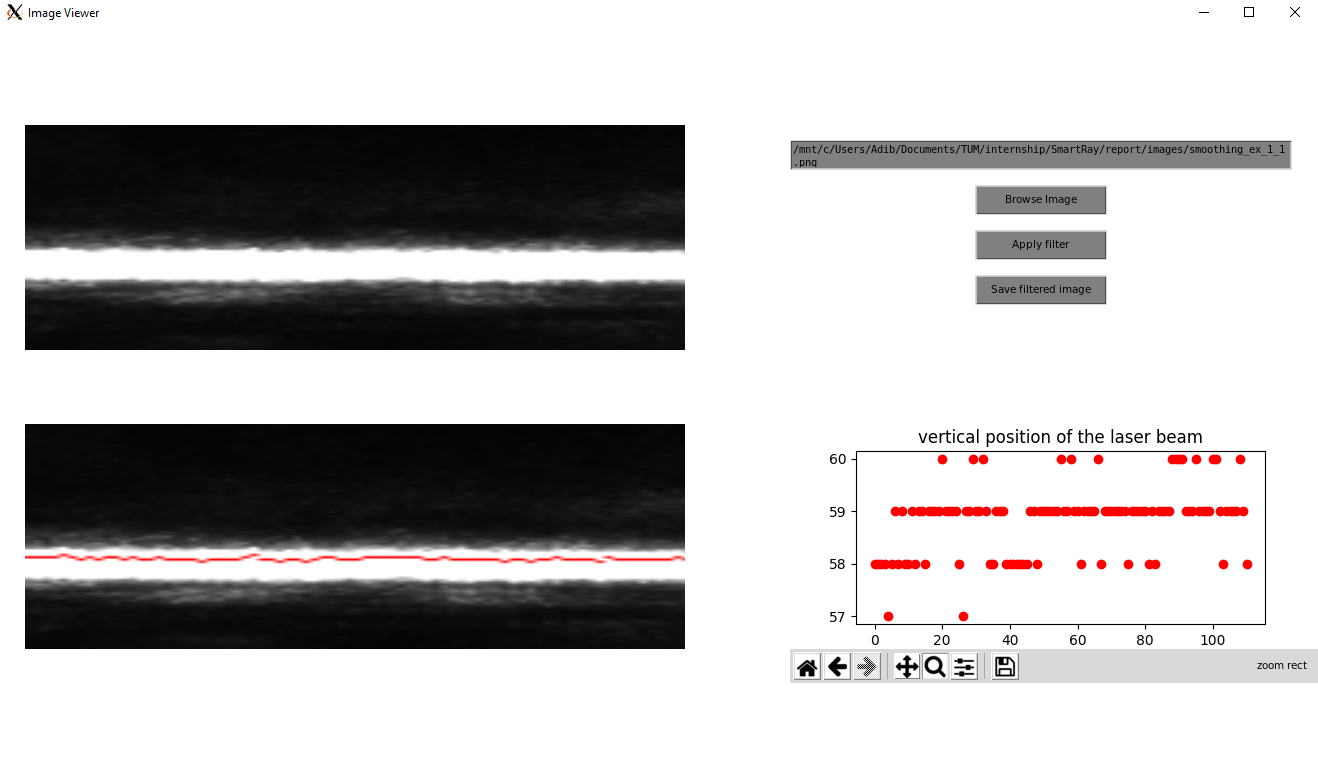
\includegraphics[width=0.8\textwidth]{image_viewer_scr_1.png}
    \caption{Image viewer tool}
    \label{fig:image_viewer_scr_1}
\end{figure}

The viewer is built using Python and TKinter with TkAgg as a rendering backend. The program is built using a mixture of OOP and functional programming paradigms. This is because of how TKinter widgets interact with each other.

Image viewer accepts only grayscale images as shown in Figure \ref{fig:image_viewer_scr_1}. In addition, the Image Viewer has slow processing time for large images because the processing is done sequentially, as concurrency isn't really optimal in Python since it doesn't provide significant speedup.


\subsection{VHDL test vector generation scripts}
\emergencystretch 4em%
    {\sloppy
        Two scripts were written to assist in executing VHDL testbenches. \lstinline{test_vector_file_gen.py} \& \lstinline{test_vector_file_data_viewer.py} are the scripts in the repository. \lstinline{test_vector_file_gen} reads image data from the \lstinline{misc} folder and exports a \lstinline{.txt} file with the correct fomatting for the \lstinline{CTRL} and \lstinline{DATA} signals. Those two signals are the inputs of the system, \lstinline{CTRL} is a 2-bit control signal (see Table \ref{tab:ctrl_table}) and \lstinline{DATA} is an 8-bit pixel value.
}

\section{VHDL code and hardware implementation}

VHDL modules within the repository are divided into their functional behaviour. Development of the VHDL system modules followed a structural design pattern, thus all of the basic digital components has been written in VHDL to ensure consistency in behaviour and avoid synthesizer ambiguity. In this section, only the major system modules will be explained. The rest are shown in Appendix A.

\subsection{FIR filter}
FIR filters are generally easy to implement in VHDL as they are only composed of multipliers, adders and basic registers. On the other hand, the decision of which architecture to implement comes with tradeoffs that depend on the general goal of the filter design. Figure \ref{fig:fir_filter_architectures} shows 4 possible filter architectures Direct FIR, Transposed FIR, pipelined Transposed FIR and Folded Direct FIR filters \cite{Akif1256720}.


\begin{figure}[h]
    \centering
    \includesvg[width=0.5\textwidth]{fir_architecture.svg}
    \caption{(a) Direct FIR, (b) Transposed FIR, (c) Pipelined Transposed FIR, (d) Folded Direct FIR}
    \label{fig:fir_filter_architectures}
\end{figure}

Direct FIR filter is the basic version of FIR filters, it is what would be basically seen in a DSP hard IP core. There is a major design shortcoming which is a very long combinational critical path from the multipliers to the output through adders as shown in Figure \ref{fig:direct_fir_filter_architectures_crit_path}


\begin{figure}[h]
    \centering
    \includesvg[width=1\textwidth]{direct_fir_filter_delay.svg}
    \caption{Critical path in Direct FIR architecture}
    \label{fig:direct_fir_filter_architectures_crit_path}
\end{figure}

The critical path delay as shown in \eqref{direct_fir_crit_path} highlights the problem with the Direct FIR design. Where $N$ is the size of the filter.


\begin{equation}\label{direct_fir_crit_path}
    \begin{aligned}
        T_{crit} = T_{mul} + (N-1) * T_{adder}
    \end{aligned}
\end{equation}

On the other hand, the Transposed FIR filter design breaks down the critical path as shown in Figure \ref{fig:transposed_fir_filter_architectures_crit_path}. The critical path delay is $T_{crit} = T_{mul} + T_{adder}$


\begin{figure}[h]
    \centering
    \includesvg[width=1\textwidth]{transposed_fir_filter_delay.svg}
    \caption{Critical path in Transposed FIR architecture}
    \label{fig:transposed_fir_filter_architectures_crit_path}
\end{figure}


The pipelined transposed FIR architecture breaks down the critical path further into being $T_{mul}$ but introduces $2*N$ more registers, where $N$ is the filter size. Also, a bigger fanout is introduced to the $X[n]$ signal as well. The introduced trade-off in the design area is a decision that has to be made. During this project, the transposed FIR filter architecture was the one implemented.

The VHDL implementation was done using generate statements which take into account the filter generic. Figure \ref{fig:fir_filter_hdl_specs} shows extensive details about the module implementation in VHDL. The data was generated using TerosHDL in vscode.


\begin{figure}[h]
    \centering
    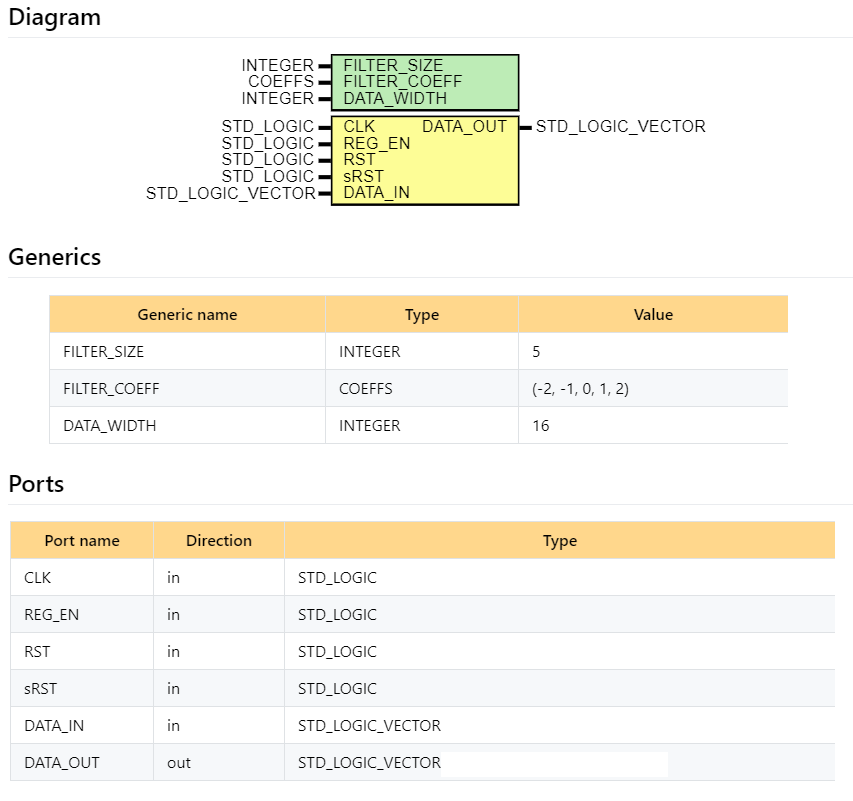
\includegraphics[width=0.8\textwidth]{fir_filter_hdl_specs.png}
    \caption{FIR filter HDL specs}
    \label{fig:fir_filter_hdl_specs}
\end{figure}

As shown in Figure \ref{fig:fir_filter_hdl_specs}, the filter coefficients, filter size and the input/output data width are generics which can be specified at module instantiation.

\subsection{Zero crossing module}

The zero-crossing algorithm is fairly simple and straight-forward to implement, since the implementation of the algorithm depends on the module finding the maximum and minimum values in the pixel column then a peak-detector module was written in VHDL. The peak-detector clocks out the index of the peak value whether it was a maximum or a minimum peak.

After the indicies of both peaks has been acquired another module ensures that the index of the maximum value is less than the index of the minimum value, because we are looking for a positive to negative going zero crossing. The module ensures that by clocking out both indicies if the values are correct, otherwise it clocks out zeros.

Finally, the zero crossing index is calculated according to \eqref{zero_index_eq}. The zero index is then clocked out of the module. Figure \ref{fig:zero_crossing_final} shows the structure of the zero-crossing module. The abundant registers are there for delay matching.


\begin{figure}[h]
    \centering
    \includesvg[width=1\textwidth]{zero_crossing_final.svg}
    \caption{Zero-crossing structural view}
    \label{fig:zero_crossing_final}
\end{figure}

Figure \ref{fig:zero_crossing_hdl_specs} shows the specifications of the zero crossing module.


\begin{figure}[h]
    \centering
    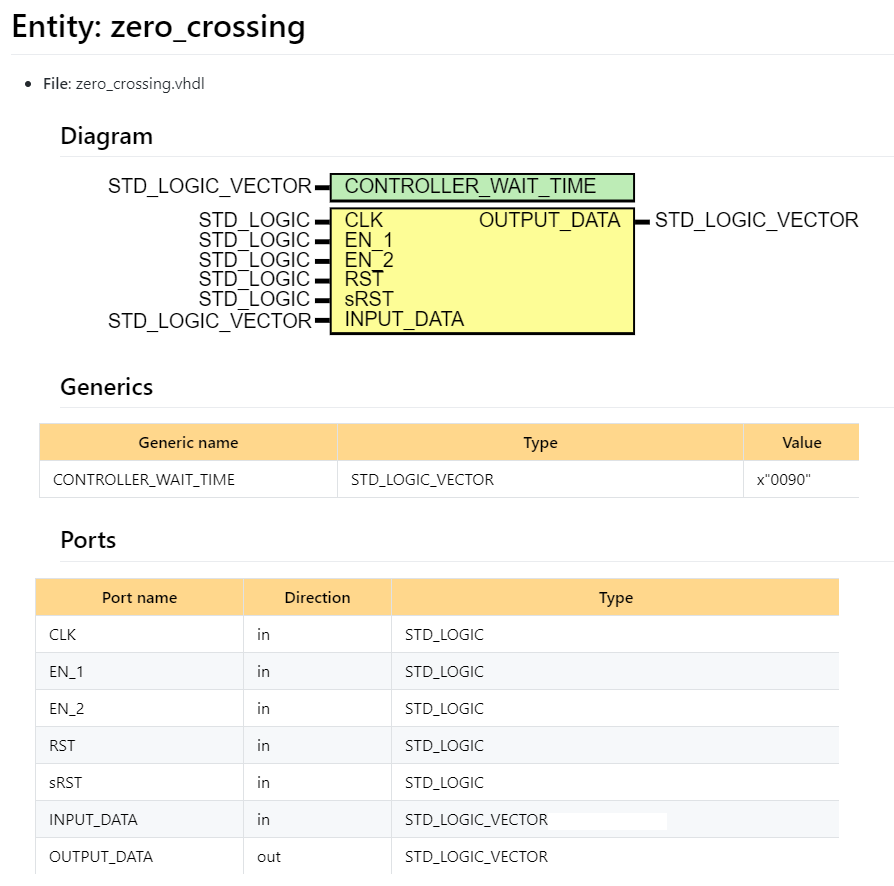
\includegraphics[width=0.6\textwidth]{zero_crossing_hdl_specs.png}
    \caption{Zero-crossing HDL specs}
    \label{fig:zero_crossing_hdl_specs}
\end{figure}

\subsection{Input controller}

The last part of the 3 major system modules is the input controller. The input controller takes the 8-bit pixel data and converts it to 16 bit. It also takes two control bits which specify the type of the data it is receiving. Table \ref{tab:ctrl_table} shows what each \texttt{CTRL} value corresponds to in terms of package type.

\begin{table}[h]
    \centering
    \begin{tabular}{ l | c }
        CTRL & TYPE  \\
        \hline \hline
        0b00 & IDLE  \\
        0b01 & START \\
        0b10 & DATA  \\
        0b11 & STOP  \\
    \end{tabular}
    \caption{Input controller control bits}
    \label{tab:ctrl_table}
\end{table}


The input controller is basically a state machine with the enable and reset signals of the system modules as its outputs. Figure \ref{fig:input_controller_hdl_specs} shows the specifications of the input controller. The module also have generics that control the timings of the output pins, the enable outputs go logic '0' when the module is flushed out of useful data.


\begin{figure}[h]
    \centering
    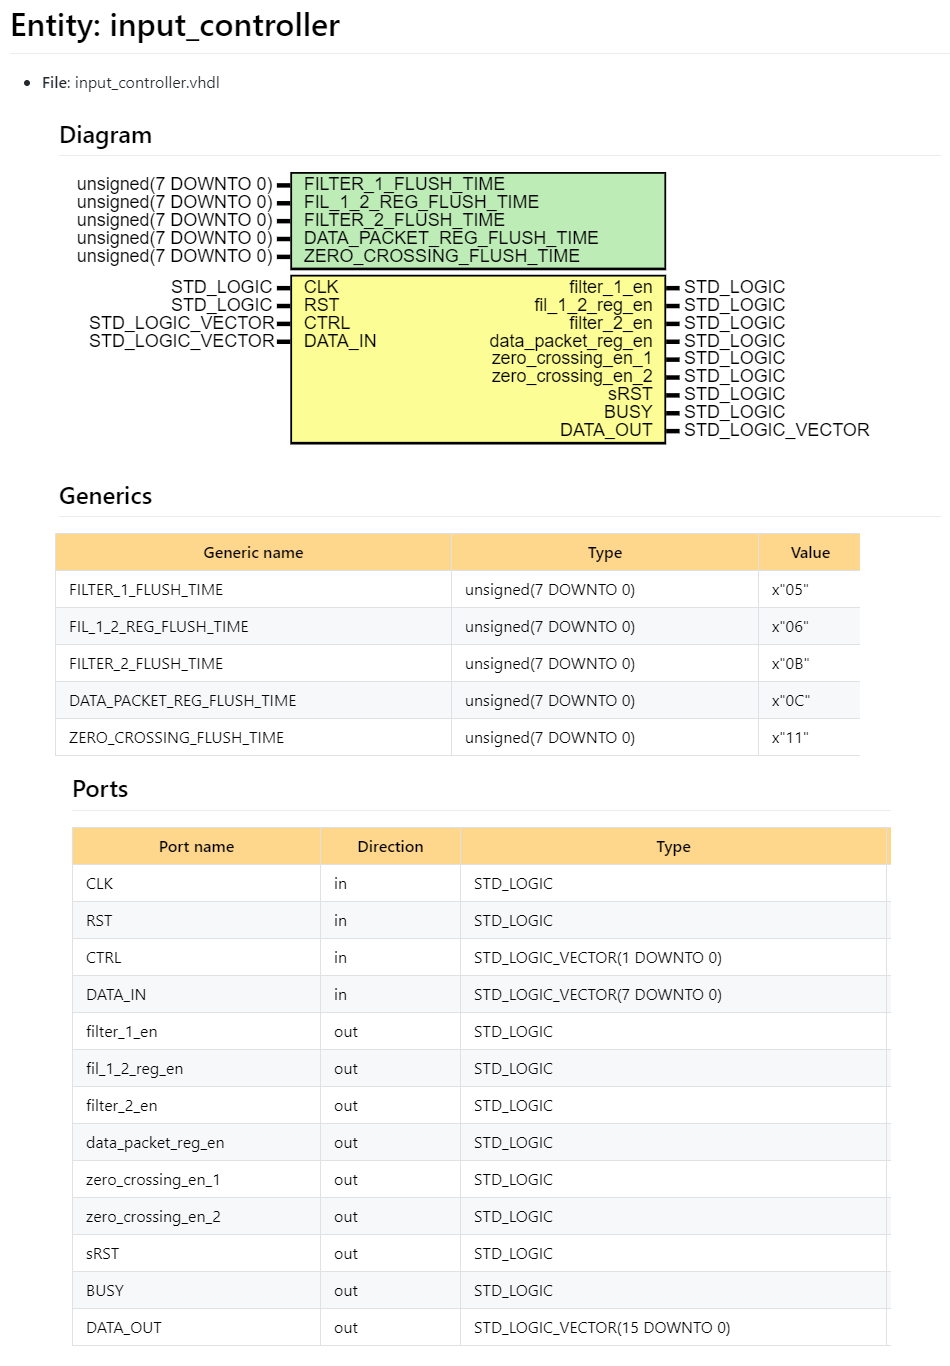
\includegraphics[width=0.8\textwidth]{input_controller_hdl_specs.png}
    \caption{Input controller HDL specs}
    \label{fig:input_controller_hdl_specs}
\end{figure}


The state machine depends on an internal counter that counts the clock cycles. Figure \ref{fig:input_controller_state_machine} shows the state diagram of the input controller's state machine.



\begin{figure}[h]
    \centering
    \includesvg[width=0.8\textwidth]{input_controller_state_machine.svg}
    \caption{Input controller state machine}
    \label{fig:input_controller_state_machine}
\end{figure}


During the \texttt{STOPPING} state, there are several conditions to check against the internal counter to disable the modules sequentially depending on the time it takes to flush those modules out.


\subsection{TOP module}

The TOP module is just a structural combination of all the aforementioned sub-system modules. Figure \ref{fig:final_sys_overview} shows the block diagram of the system. The index counter module is basically a counter that starts counting after a specified delay. This module is used to combine the delayed output data from the filters with their indicies so they can be used in the zero crossing module.


\begin{figure}[h]
    \centering
    \includesvg[width=0.8\textwidth]{final_sys_overview.svg}
    \caption{Block diagram of TOP}
    \label{fig:final_sys_overview}
\end{figure}

\section{Build system}

The VHDL code analysis, elaboration and simulation are all done using GHDL. The main appeal of the tool is the ability of working with VHDL modules from the terminal. GHDL allows the user to generate a wave \texttt{.vcd} file, the wave file can be viewed using GTKWave.

To automate the process of code analysis, elaboration, and simulation Make was used. The MakeFile is located in the build folder in the repository where all the compiled binaries are located as well. The MakeFile also provides some other functionality to the user such as viewing the wavefiles in GTKWave.


\chapter{Conclusion}

\section{Results discussion}

The system processes data from the image sensor one pixel column at a time. In each processed pixel column the zero-crossing module will find an index where the zero-crossing happens, this index is the location of the point of maximum intensity on the laser line. Figure \ref{fig:filtered_ex_result_1} shows the result of passing an image through the system. The red line highlights the points of maximum intensity detected by the system.


\begin{figure}[h]
    \centering
    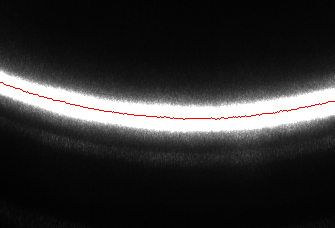
\includegraphics[width=0.4\textwidth]{filtered_ex_result_1.png}
    \caption{Example processing result}
    \label{fig:filtered_ex_result_1}
\end{figure}


The system produces accurate results when the images are not noisy nor highly exposed. The fix for noise was addressed by the use of a smoothing filter. But the high exposure produces high intensity patches in the image as shown in Figure \ref{fig:high_exposure_img_ex_1}. The patches skew the result of the zero-crossing detector as well. This is due to the fact that the patches are of saturated intensity which makes it hard for the smoothing filter to get rid off.


\begin{figure}[h]
    \centering
    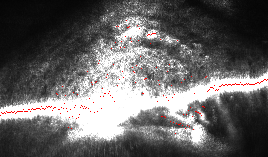
\includegraphics[width=0.5\textwidth]{high_exposure_img_ex_1.png}
    \caption{Skewed results due to over-saturated areas}
    \label{fig:high_exposure_img_ex_1}
\end{figure}


Figure \ref{fig:high_exposure_img_ex_2} shows how the pixel column looks like when the image is exposed for too long. It also shows the detected index is shifted due to the high distortion in the image. A solution to this problem would be to adjust the exposure time according to the material being scanned.


\begin{figure}[h]
    \centering
    \includesvg[width=0.5\textwidth]{high_exposure_img_ex_2.svg}
    \caption{Highly exposed image next to graph of raw and differentiated data}
    \label{fig:high_exposure_img_ex_2}
\end{figure}




\section{Next steps}
\subsection{System optimization}

The design has been implemented in VHDL and its functional behavior has been verified. Afterwards, the design was synthesized for an Intel Cyclone V and achieved a maximum frequency of 228 MHz. However, further speed improvements can be done to increase the clock frequency further. Such as the use of approximated multipliers.

\subsection{Data threshold}

The differentiation filter and the zero-crossing algorithm work better when the noise is eliminated completely from the input pixel data. A method which was tested in the Python script was to cull the data which is below a certain threshold, 80\% of the maximum value is a dataset provided very good results. The issue with this method is that the maximum value is not known beforehand which means that the system needs to read all the values first then calculate 80\% of that value then cull the data points below that value. This introduces large latencies to the system. So, a set threshold or a dynamic threshold could be used on a frame-to-next-frame basis.



\backmatter
% optional: list of figures
\listoffigures
% optional: list of tables
% \listoftables
% % optional: list of source code listings
% \lstlistoflistings

% your BibTex file
\bibliography{bib/references.bib}


\appendix
% include appendix chapters here

\chapter{Appendix A}
\section{VHDL module specifications}

\subsection{Adder}

\begin{figure}[h]
    \centering
    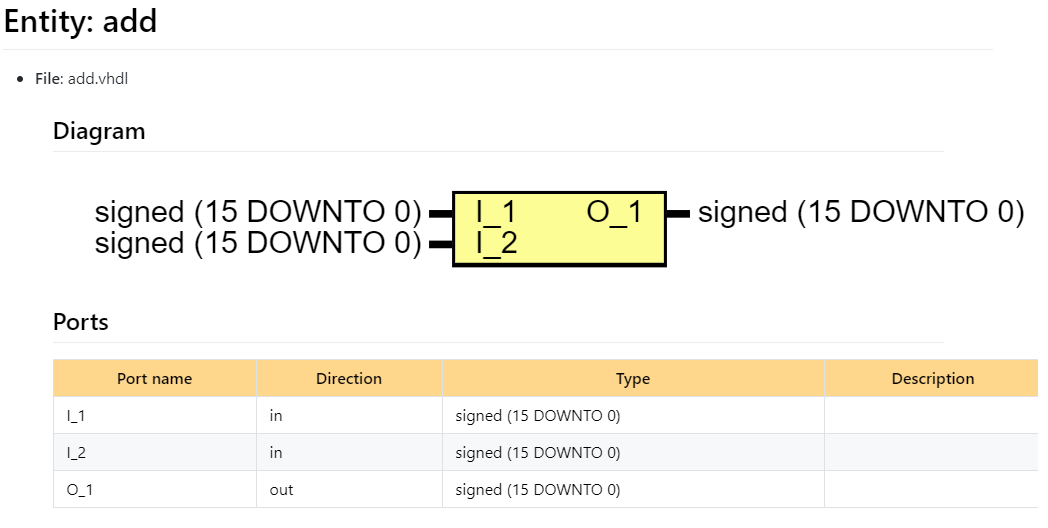
\includegraphics[width=0.9\textwidth]{adder_specs.png}
    \caption{Adder specifications}
    \label{fig:adder_specs}
\end{figure}

\subsection{Multiplier}

\begin{figure}[h]
    \centering
    \includegraphics[width=0.9\textwidth]{Mul_specs.png}
    \caption{Mul specifications}
    \label{fig:mul_specs}
\end{figure}

\subsection{D-FlipFlop}

The D-FlipFlop supports both synchronous and asynchronous resets.

\begin{figure}[h]
    \centering
    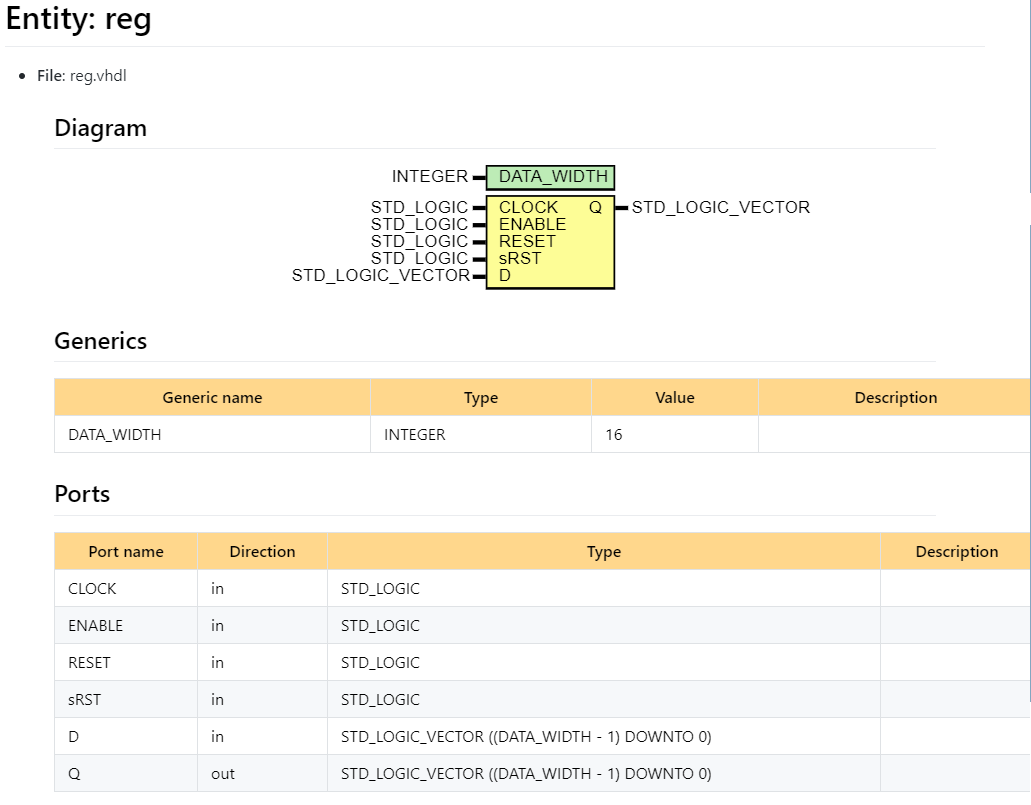
\includegraphics[width=0.6\textwidth]{reg_specs.png}
    \caption{FlipFlop specifications}
    \label{fig:reg_specs}
\end{figure}

\subsection{Peak Detector}

\begin{figure}[h]
    \centering
    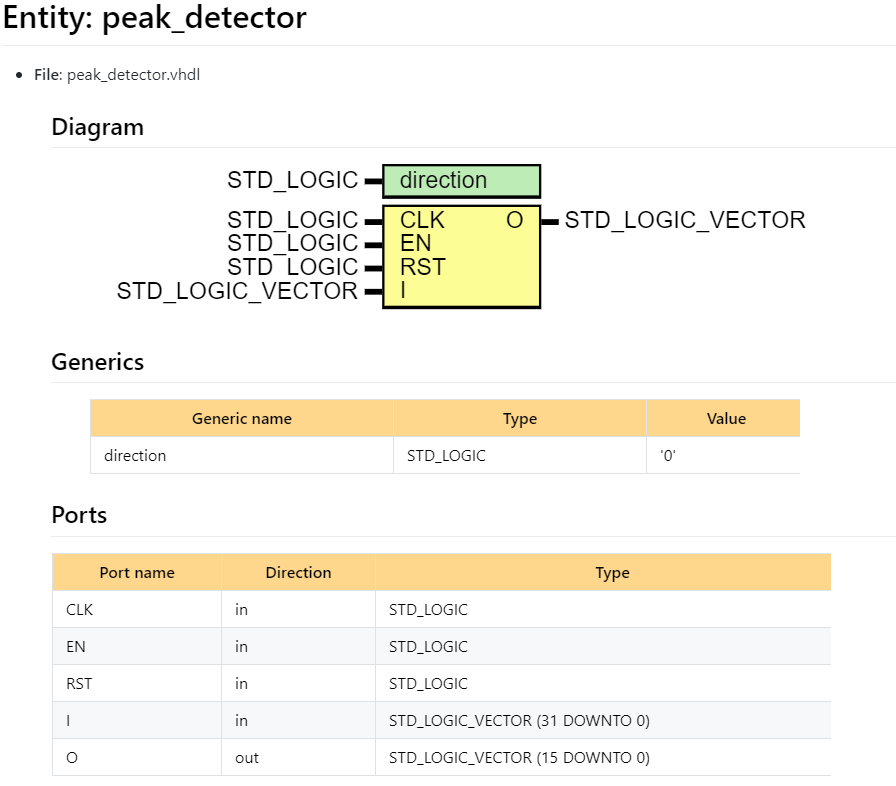
\includegraphics[width=0.6\textwidth]{peak_specs.png}
    \caption{Peak Detector specifications}
    \label{fig:peak_specs}
\end{figure}





\end{document}
